\part{Session 1}

\section{Introduction}
\subsection{What is mbed}
\begin{frame}
	\frametitle{What is mbed}
	The mbed development platform is a collection of open source hardware and software to allow rapid ARM based prototyping.
	\begin{itemize}
		\item Professional online compiler lets you work from any computer
		\item Integrated version control system lets you easily find and use open source libraries
		\item CMSIS based APIs for core and peripheral functions let you work high level or bare metal
		\item Hardware abstraction layer insulates your application code from hardware changes
	\end{itemize}
	\textit{Essentially a high performance Arduino with highly integrated tools to save you time}
\end{frame}

\begin{frame}
	\frametitle{Register on mbed}
	\begin{columns}[c]
		\begin{column}{0.5\textwidth}
			%TODO Edit mbed_register
			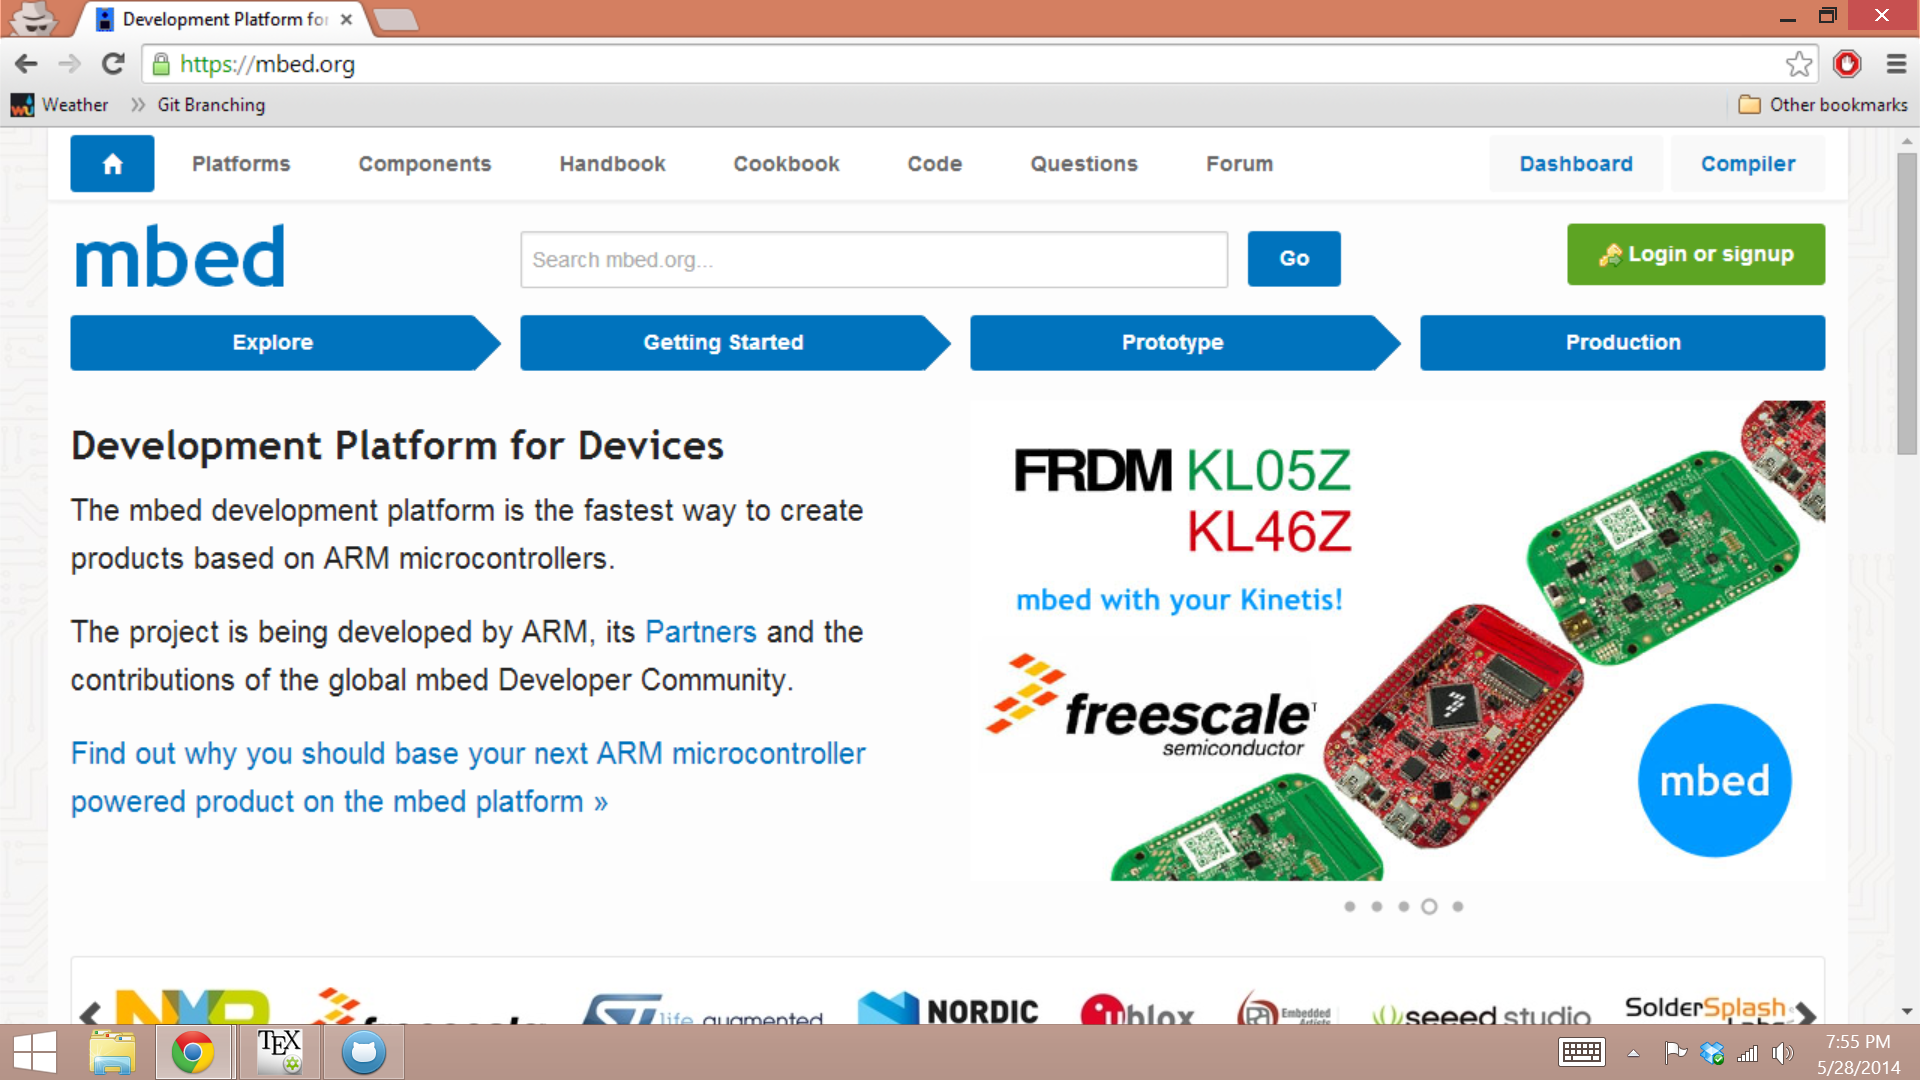
\includegraphics[width=\linewidth]{mbed_register}
		\end{column}
		\begin{column}{0.5\textwidth}
			\begin{enumerate}
				\item Navigate to \url{http://www.mbed.org}
				\item Click the green login or signup button
				\item Click the signup button
				\item Follow the prompts
				\item Confirm your e-mail address
			\end{enumerate}
		\end{column}
	\end{columns}
	\vspace{1ex}
	Everyone should have an account on mbed.
	You can create a team to share programs between users in your organization.
\end{frame}

\subsection{Nucleo Development Board}
\begin{frame}
	\frametitle{Nucleo Development Board}
	\begin{columns}[T]
		\begin{column}{0.5\textwidth}
			The Nucleo development board combines a USB programmer with a powerful STM32 processor and Arduino compatible headers
			\begin{itemize}
				\item ARM Cortex-M4 with FPU at 84 MHz
				\item 512 KBytes flash memory
				\item 12bit ADC at 2.4 Msps with up to 10 channels
				\item Up to 3xUART, 3xI2C, 4xSPI interfaces
			\end{itemize}
		\end{column}
		\begin{column}{0.5\textwidth}
			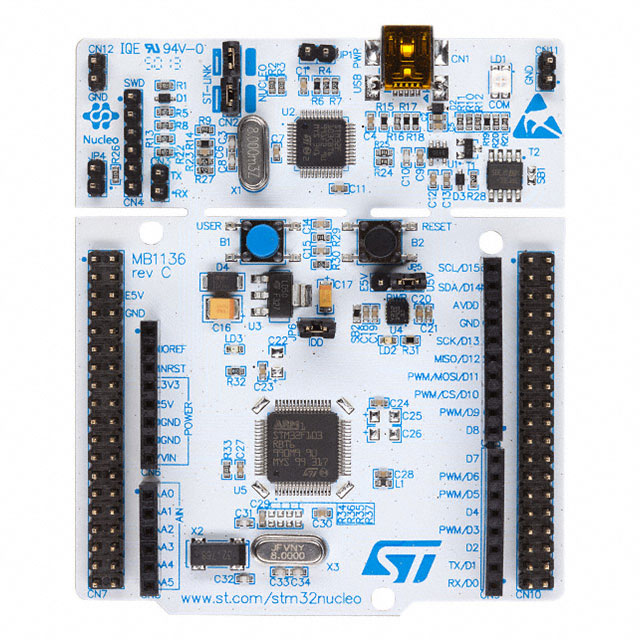
\includegraphics[width=\linewidth]{nucleo}
		\end{column}
	\end{columns}
\end{frame}

\begin{frame}
	\frametitle{Add Nucleo to Your Account}
	\begin{columns}[c]
		\begin{column}{0.5\textwidth}
			%TODO Edit add_nucleo
			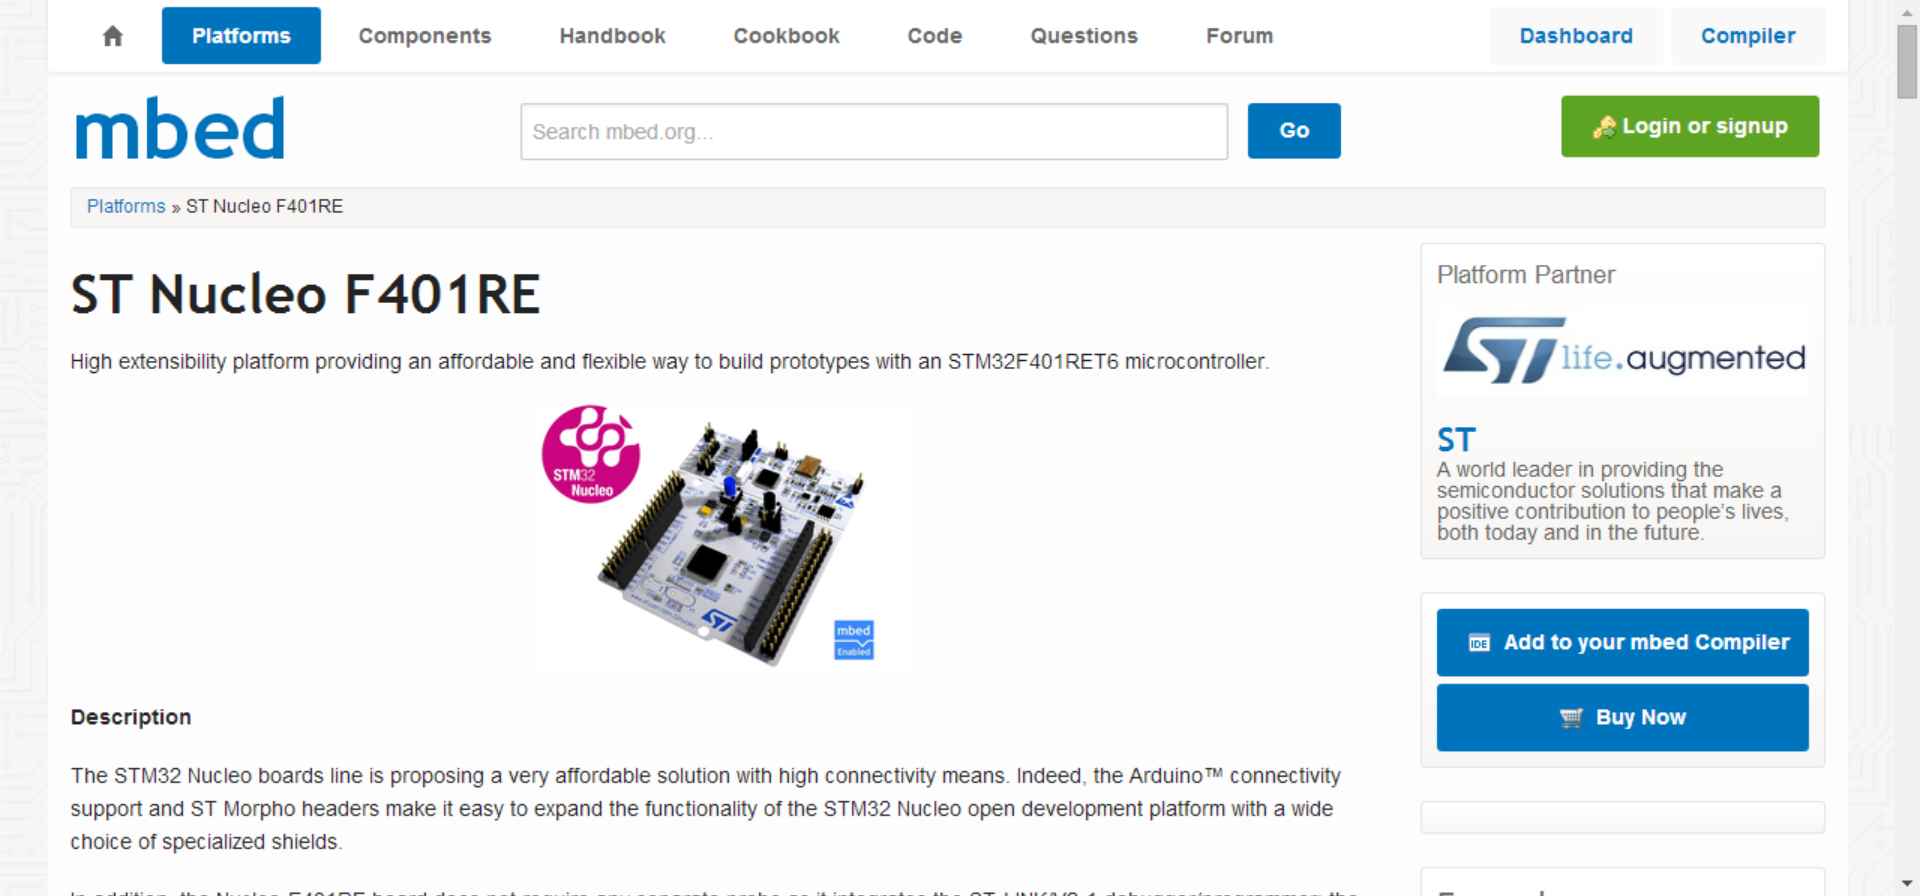
\includegraphics[width=\linewidth]{add_nucleo}
		\end{column}
		\begin{column}{0.5\textwidth}
			\begin{enumerate}
				\item Connect your Nucleo to your computer
				\item Open the external drive that connects
				\item Open the mbed.htm file
				\item Click "Add to Your mbed Compiler"
				%TODO add nucleo to compiler steps
			\end{enumerate}
		\end{column}
	\end{columns}
	\begin{block}{Notice}
		You only need to do this once!
	\end{block}
\end{frame}

\subsection{An Example Program}
\begin{frame}
	\frametitle{An Example Program}
	\begin{columns}[T]
		\begin{column}{0.5\textwidth}
			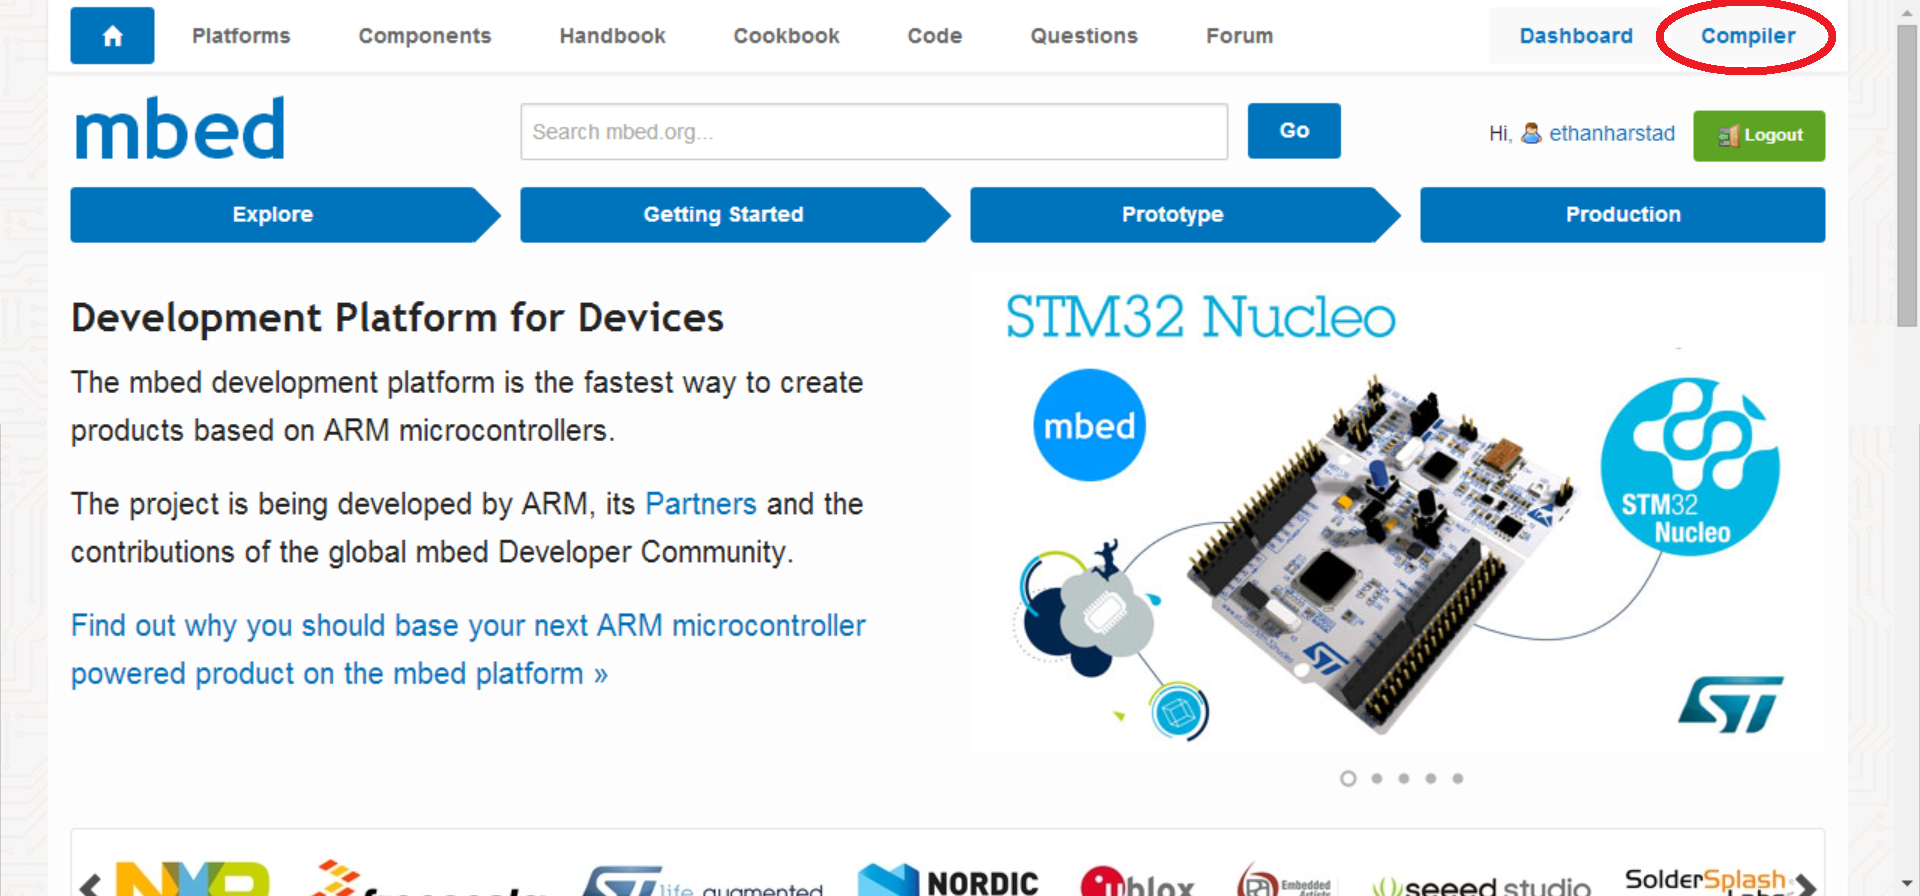
\includegraphics[width=\linewidth]{open_compiler}
			\vspace{1ex}
			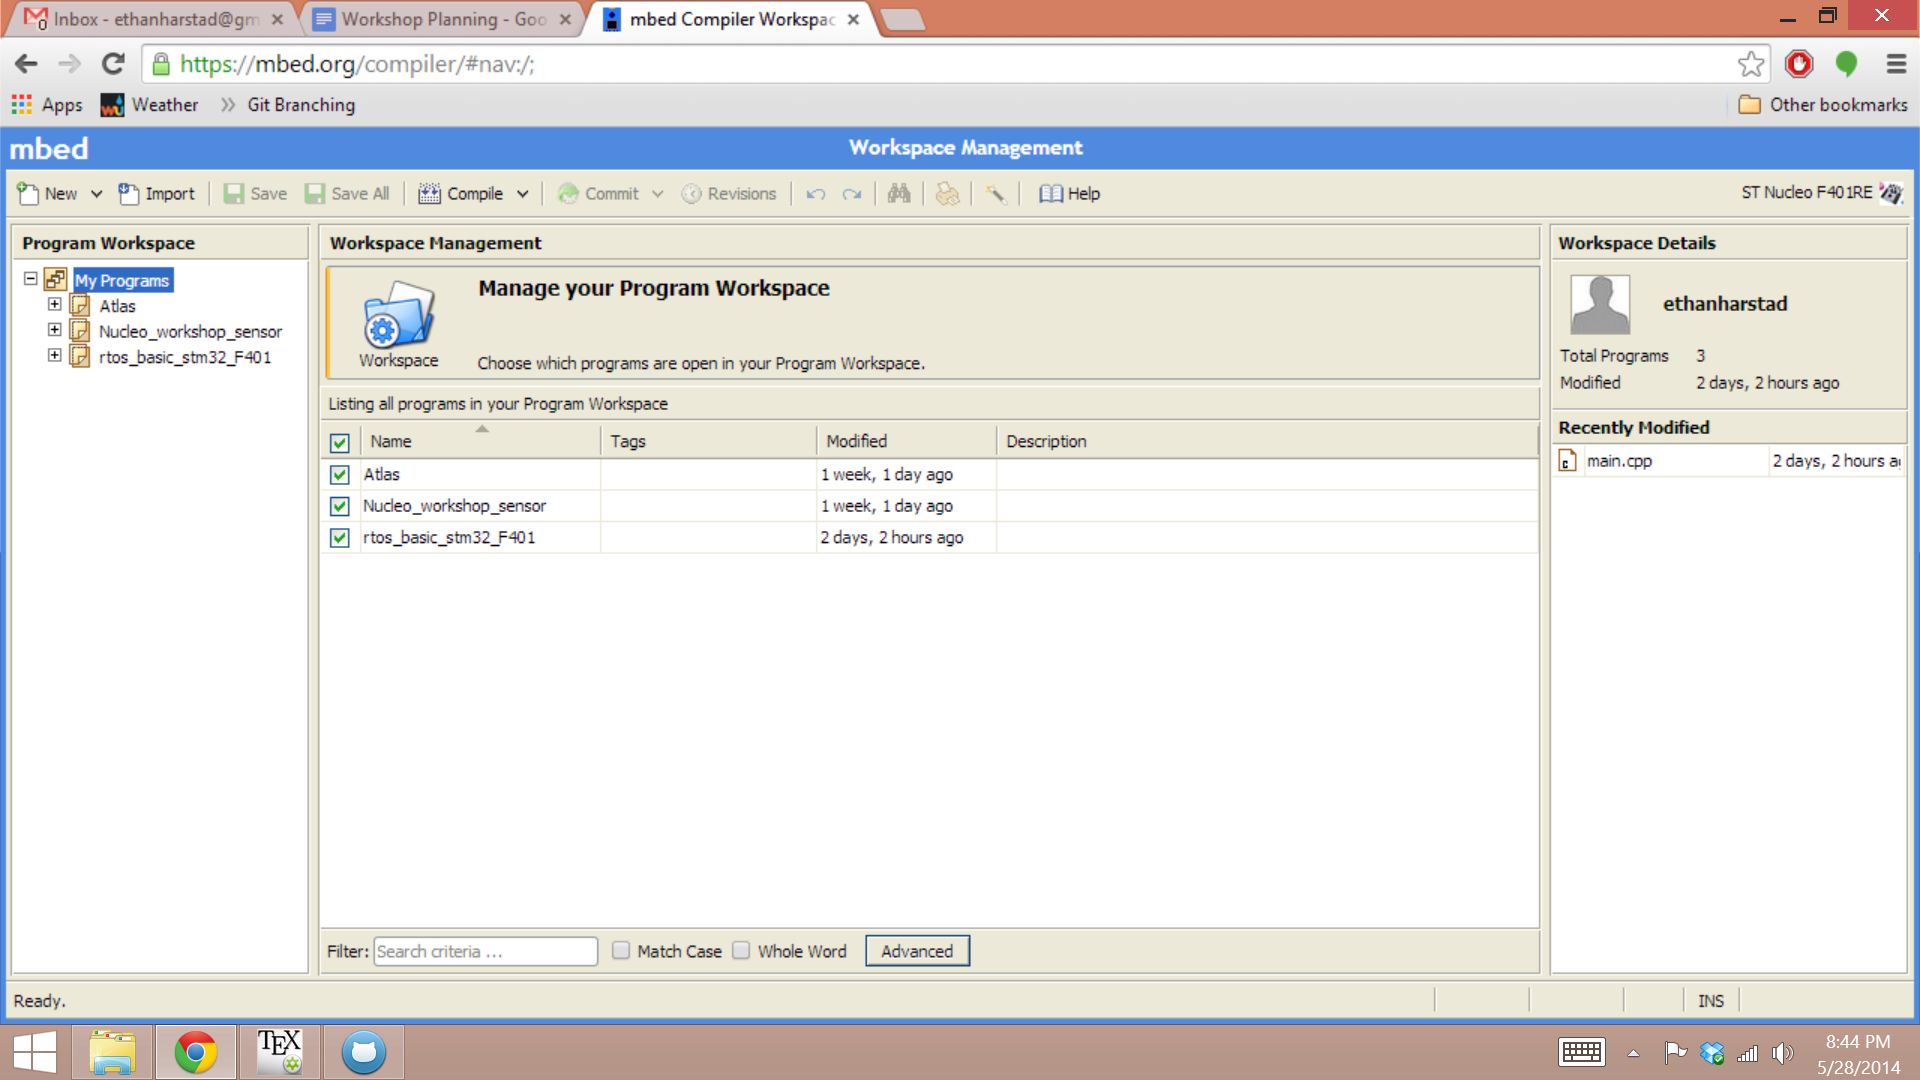
\includegraphics[width=\linewidth]{new_project}
		\end{column}
		\begin{column}{0.5\textwidth}
			\begin{enumerate}
				\item Navigate to \url{http://www.mbed.org}
				\item Click the Compiler button
				\item Click New and select New Program
				\item Choose "Blinky LED" as the program template
				\item Name the program anything you desire and click OK
			\end{enumerate}
		\end{column}
	\end{columns}
\end{frame}

\begin{frame}
	\frametitle{Compile and Upload Your Program}
	\begin{columns}[T]
		\begin{column}{0.5\textwidth}
			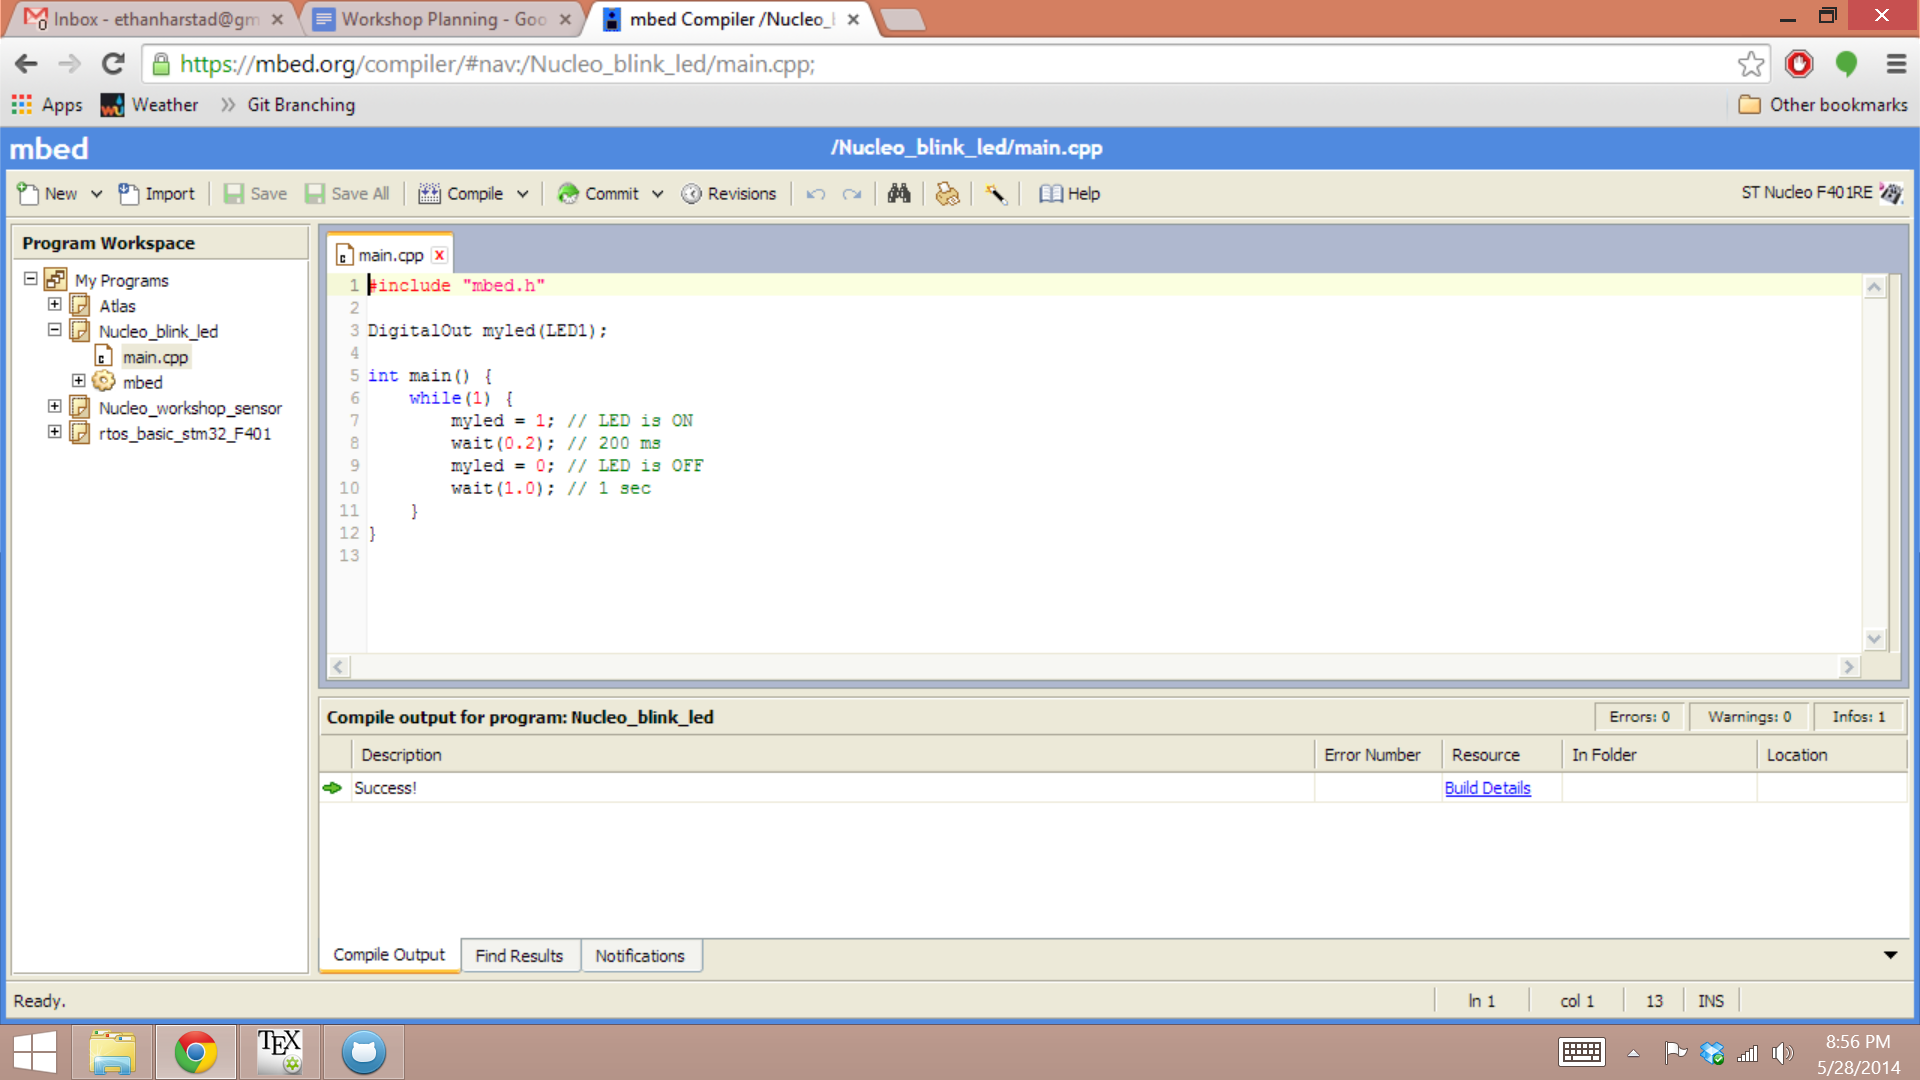
\includegraphics[width=\linewidth]{compile_program}
			\begin{block}{Tip}
				Set your browsers download location to the Nucleo to save time while debugging
			\end{block}
		\end{column}
		\begin{column}{0.5\textwidth}
			\begin{enumerate}
				\item Click Compile
				\item A file will be downloaded
				\item Move this file to the Nucleo external drive
				\item The LED will flash red/green while programming
				\item When the` LED is solid green, your program has started successfully!
			\end{enumerate}
		\end{column}
	\end{columns}
\end{frame}